\documentclass[modern]{aastex63}

% \received{June 1, 2019}
% \revised{January 10, 2019}
% \accepted{\today}
% \submitjournal{AJ}

% \shorttitle{Sample article}
% \shortauthors{Schwarz et al.}
% \watermark{DRAFT}
% \setwatermarkfontsize{dimension}

\usepackage[super]{nth}
\usepackage[inline]{enumitem}

\renewcommand{\vec}[1]{\mathbf{#1}}
\newcommand{\fracpartial}[2]{\frac{\partial #1}{\partial #2}}
\newcommand{\Lsun}{\mathrm{L_\odot}}
\newcommand{\ledd}{L_{\mathrm{Edd}}}
\newcommand{\Rsun}{\mathrm{R}_\odot}
\newcommand{\Msun}{\mathrm{M}_\odot}
\newcommand{\emphbf}[1]{\textbf{\emph{#1}}}
\newcommand{\kms}{\mathrm{km~s^{-1}}}
\newcommand{\kev}{\mathrm{keV}}
\newcommand{\eV}{\mathrm{eV}}
\newcommand{\cmcub}{$\mathrm{cm}^{-3}$}
\newcommand{\msyr}{\mathrm{M_{\odot}}~\mathrm{yr^{-1}}}
\newcommand{\cm}{\mathrm{cm}}
\newcommand{\s}{\mathrm{s}}
\newcommand{\km}{\mathrm{km}}
\newcommand{\gm}{\mathrm{gm}}
\newcommand{\K}{\mathrm{K}}
\newcommand{\g}{\mathrm{g}}
\newcommand{\G}{\mathrm{G}}
\newcommand{\AU}{\mathrm{AU}}
\newcommand{\erg}{\mathrm{erg}}
\newcommand{\ergsec}{\mathrm{erg~s^{-1}}}
\newcommand{\yrs}{\mathrm{yrs}}
\newcommand{\yr}{\mathrm{yr}}
\newcommand{\pc} {\rm{pc}}
\newcommand{\kpc}{\mathrm{kpc}}
\newcommand{\Mpc}{\mathrm{Mpc}}
\newcommand{\etc}{$\eta$~Car}
\newcommand{\days}{\mathrm{days}}
\newcommand{\keV}{\mathrm{keV}}
\newcommand{\jd}{\mathrm{JD}}
\newcommand{\mjd}{\mathrm{MJD}}
\newcommand{\Ha}{\mathrm{H}\alpha}

\begin{document}

\title{The Energy Time Diagram and the Relation to Intermediate Luminosity Optical Transient}

% \correspondingauthor{Amit Kashi}
\email{amirmi@ariel.ac.il, kashi@ariel.ac.il}

\author[0000-0002-1361-9115]{Amir Michaelis}
\affiliation{Department of Physics, Ariel University, Ariel, POB 3, 4070000, Israel}

\author[0000-0002-7840-0181]{Amit Kashi}
\affiliation{Department of Physics, Ariel University, Ariel, POB 3, 4070000, Israel}

\begin{abstract}
The Energy Time Diagram is a way to present transient.
Each point represents the total energy and duration of the transient.
Focus on Intermediate Luminous Optical Transients (ILOTs) the location of such objects in the EDT form a strip, the Optical Transient Stripe (OTS).
We update the ETD to include latest observation of ILOTs and suggest classification of the objects by the location in the OTS.
\end{abstract}

\keywords{accretion, accretion disks --- (stars:) binaries: general --- stars: mass-loss 
--- (stars:) supernovae: general 
---  stars: variables: general}

\section{Introduction} \label{sec:intro}
Analyzing the light curve of erupting object is imported to understand the nature of the transient.
We can deduce a lot of information only from the light cure.
When plotting the light curve of a collection of objects we see similarities between different groups for example nova or Super Nova (SN) type Ia and more.
We also have a certain objects that at first glance classified as one of the groups, but after more examination it does not fit to any of the groups.
These special transients that sometimes called super nova imposters have similar light curve shape after scaling the time axis \citep{2010ApJ...709L..11K}.
Anther way to present these objects is by using the Energy Time Diagram \citep[ETD; ][]{2010arXiv1011.1222K}.
In this diagram we plot the total energy of the transient (radiation plus kinetic energy) vs the total duration.
When we do so we see that all this objects we shell now call Intermediate Luminous Optical Transients (ILOTs) form a slated stripe more energetic than novae yet less energetic than SNe referred to as the Optical Transient Stripe (OTS).
This behavior suggests that ILOTs have a similar powering mechanism. 
The most feasible mechanism is gravitational processes (for example \citealt{2016RAA....16...99K}).
Example for relevant gravitation dominated process can be accretion thick disc, binary system merger, binary system with extreme eccentric orbit, giant eruption, young stellar object outburst and more.
The ILOTs physical scenario is quite diverse \citep{2018Galax...6...82K}.
We discuss the common properties of ILOTs, and heir types.
Then we update the EDT to include the following conform objects \cite{2016ApJ...826..191H,2018MNRAS.480.3424C,2018MNRAS.473.4805K,2019A&A...632L...6C,2019A&A...625L...8P,2019ApJ...880L..20J,2019ApJ...887..169H,2019Galax...8....2K,2019A&A...621A..30S,2020MNRAS.492.5897S}.
Next We will present the light curve of the transients and show the similarities (after scaling the time axis).
And discuss the use of ETD and light curve to help classified the transient as an ILOT object.

%%%%%%%% other use of ILOTs name and types 
\subsection{Types of ILOTs \label{subsec:Types of ILOTs}}

We summaries the different scenarios that occupies the OTS in the ETD.
This scenarios are quite divers and wide including objects that range from brown dwarfs to very massive stars.
The classification and naming we use here follow \citep{2018Galax...6...82K} but there is still no consensus regarding the naming for example \cite{2019ApJ...886...40J,2019A&A...630A..75P}.

\begin{itemize}

\item \label{lrn-ilot-item} \emphbf{Luminous Red Nova (LRN) or Red Transients (RT) or Merger-Burst.} 
These group describe transient powered by merger of two stars.
The denser star tidally destroys the less dense star and accretes most of its mass. 
This releases gravitational energy that powers the event. 
Some mass from the destroyed star escapes the system.
The most famous examples for LRN is V838~Mon \citep{2005A&A...441.1099T}.

\item \label{ilrt-ilot-item} \emphbf{Intermediate Luminosity Red Transients (ILRT).} 
In this group a star in the Asymptotic Giant Branch (AGB) or Red Giant Branch (RGB) experience an ILOT event, most probable powered by gravitational energy of a companion that accretes mass from the giant star at a very high rate. 
Example for this scenario is SN~2008S \citep{2009ApJ...697L..49S,2009ApJ...705.1425P,2010MNRAS.403..474W,2016MNRAS.462..217S}.

\item \label{ges-ilot-item} \emphbf{Giant Eruptions (GEs).} 
These are eruptions of Luminous Blue Variables (LBVs) or other kinds of very massive stars for example Wolf-Rayet starts, o-type and others, usually observe as atypical SN or SN impostors.
The typical scenario here is a binary system with extreme eccentric orbit where we cannot see the companion because of dust obscuring.
Giant eruptions ILOTs typically characterize with the high energy relative to other classes (a few $\times10^{49} \erg$) and consider the high mass relatives of ILRTs. 
There are two famous events is this group \etc eruption in the \nth{19} century \citep{2010ApJ...723..602K} and P~Cyg eruption in the \nth{17} century \citep{2010ApJ...723..602K,2018NewA...65...29M} 

\item \label{pne-ilot-item} \emphbf{ILOTs which created Planetary Nebulae (PNe).} 
We suggest that one possible scenario for creating planetary nebula is through ILOT event lasting up to a few months.
For more details on this possibility see the high accretion powered ILOT model \citep{2016RAA....16...99K} and the simulation by \cite{2013MNRAS.436.1961A}.
An example for this scenario is the bipolar PN~NGC~6302.

\item \label{plant_and_bd-ilot-item} \emphbf{Weaker Merger-burst between a Planet and a Brown Dwarf.} 
According to this suggested scenario, a planet or a brown dwarf is shredded into a disk around a brown dwarf or a star respectively and the energy from accretion leads to an outburst \citep{2011MNRAS.416.1965B}. 
The process is a super-Eddington merger-burst that resides in the lower part of the OTS on the ETD.
If we consider the following scenario of plant and brown dwarf where the orbit of the planet is perturbed to reduce the periastron distance, such that the planet gets into the tidal radius at periastron the planet will destructed by the brown dwarf and as a result the remnant will resemble LRNs but on shorter time scale and smaller energy.

\item \label{yso_outburst-ilot-item} \emphbf{A Weak Outburst of a Young Stellar Object (YSO).} 
In this suggested scenario a young stellar object undergo unusual outbursts for example ASASSN-13db \citep{2017A&A...607A.127S,2019Galax...8....2K}.
This outbursts are similar in many aspects to LRNe events but with lower total energy (and much fainter). 

\end{itemize}

The above types of ILOTs can also be classified according to the angle from were they are observed \citep[in a similar manner to the classification of galaxies and active galactic nuclii;][]{2015ARA&A..53..365N}:

\begin{itemize}

\item \label{type_i-ilot-item} \emphbf{Type I ILOTs.} 
ILOTs which are directly observed. 
The condition for an ILOT to be classified as type I is that the observing direction is such that the ILOT is not obscured from the observer by an optically thick medium.

\item \label{type_ii-ilot-item} \emphbf{Type II ILOTs.}  
Since most ILOTs are non-spherically symmetric eruptions we can expect that the same transient will appear differently only as a result of the point of view in the sky \citep{2017MNRAS.467.3299K}. 
This brings a new ILOT type, the Type II ILOTs.
The main property of this type is its orientation which makes the photosphere of the ILOT to be obscured.
Namely, the line of sight to the object intersects with a thick dust torus or an optically thick cloud.
A possible formation scenario can be a strong tidal interaction at periastron passage in an eccentric orbit. 
The interaction leads to an axisymmetrical mass ejection which significantly departs from spherical symmetry.
If the light from the object is severely attenuated or hidden we will classified it as type II.
In most cases, the obscuring matter would reside in equatorial directions. 
The binary system will be obscured to the observer in the optical and IR bands as long as the dust has not dissipated.
A type II ILOT is accompanied by some polar mass ejection that may also form dust.
The dust in the polar directions interacts with the radiation that arrives from the central source.
We then can observe this reflected light which becomes much fainter and by doing so allowing the type II ILOT to be detectable. 
A possible example is the outburst of the red supergiant N6949-BH1 in 2009 \citep{2017MNRAS.468.4968A}.

\end{itemize}

\section{Observation}
Optional method to report transient event is by the event peck luminosity \citep{2013IAUS..281....9K,2020MNRAS.492.3229H}, but this method is falling short as the total energy that is radiation energy plus gravitation energy is needed in order to fully classified the event.  
Next we summaries the main observational properties of the objects we used to update the ETD to get a more complete picture in focus, of course, on the total energy.

\subsection{Massive Star Giant Eruption Outflows of PSN~J09132750+7627410 in NGC~2748}
The object PSN~J09132750+7627410 (hereafter PSNJ09+76) first reported as possible supernova (PSN) 2015 February 10 at the IAU Central Bureau for Astronomical Telegrams (CBAT\footnote{\url{http://www.cbat.eps.harvard.edu/unconf/followups/J09132750+7627410.html}}).
On 2015 February 12 it was classified as supernova imposter \citep{2015ATel.7051....1T}.
PSNJ09+76 is member of the galaxy NGC~2748 that is part of the NASA/IPAC Extragalactic Database (NED\footnote{\url{http://ned.ipac.caltech.edu/}}) survey \citep{2017AJ....153...37S} with mean distance of $22.23 \pm 1.56 \Mpc$. 
Follow-up multicolor photometric and spectrum \citep{2016ApJ...823L..23T,2016ApJ...826..191H} estimate the outburst peak luminosity at $\sim 10^{41} \ergsec$.
From spectroscopic analysis PSNJ09+76 as $\Ha$ P~Cyg profile with velocities $\sim 700 \kms$.
At all phases the spectra of PSNJ09+76 are characterized by prominent Balmer $\Ha$ emission lines showing sharp and narrow P~Cygni profiles.
Two absorption components suggests the presence of two expandind shaells moving at different velocities $\sim 1000 \kms$ and $\sim 340-450 \kms$.
progenitor observation suggest most likely solar metallicity with effective temperature of $\sim 7250\K$ luminosity of $\log(\mathrm{L}/\Lsun)\simeq 5$ mass $\sim 25 \Msun$ supergiant OH/IR type star

\subsection{Luminous Red Nova AT~2017jfs in NGC~4470}
bolometric luminosity $5.5\times10^{41}\ergsec$
common envelope transient merger of massive binary event
galaxy NGC~4470 face on early type spiral galaxy, mean distance $18\pm6.6\Mpc$ NASA/IPAC Extragalactic Database (NED\footnote{\url{https://ned.ipac.caltech.edu/}}) kinematic distance $d\sim 35.2\pm 2.7 \Mpc$ estimate by \cite{}\dots
object alias names Gaia17dkh PS17fqp ATLAS18aat
The maximum peck in g-band (very similar to V-band)  $M_g=-15.46 \pm 0.15 $ observed at $\mjd = 58114.8 \pm 1.8 $ (2017 December 27.8 UT) 
spectrum blue continuum dominated by prominent H lines in emission with a Lorentian profile with velocities of $\sim 700 \kms$ 
with time the H lines become fainter and show $\Ha$ P~Cygni profile.
The late time spectrum suggest an late G to K types star.
A spectrum after 5 months suggest the object is an M type star with velocities of $400\kms$
$L\sim 5.5^{41}\times\ergsec$ 
We discuss .... \cite{2019A&A...625L...8P}

\subsection{Intermediate Luminosity Red Transient AT~2019abn in M51}
Messier 51
M51~OT2019-1 also ZTF~19aadyppr, AT~2019abn, ATLAS19bzl
cite ZTF \cite{2019PASP..131a8002B,2014htu..conf...27B} \dots
during the outburst show a red continuum Balmer emission with velocity width of $\approx 400\kms$ and F-type supergiant typical absorption and emission.
spectra and multiband light curve similar to other ILOTs.
The progenitor is similar to SN~2008S and NGC~300~OT2008-1.
event observed in MESSIER~51 (the Whirlpool galaxy) at $8.58\pm0.10\Mpc$ \citep{2016ApJ...826...21M}
The event first observed at MJD=58505.6 (UT 2019 January 22.6) 
%http://www.growth.caltech.edu Global Relay of Observatories Watching Transients Happen (GROWTH)

We discuss .... \cite{2019ApJ...880L..20J} \\
We discuss .... \cite{2020arXiv200108782W}

\subsection{SN2018gep}
We discuss .... \cite{2019ApJ...887..169H}

\subsection{ASASSN-13db 2014-2017 Eruption as an Intermediate Luminosity Optical Transient}
We discuss .... \cite{2019Galax...8....2K}

\subsection{iPTF14hls}
We discuss .... \cite{2019A&A...621A..30S} 

\subsection{MCA-1B WR LBV}
We discuss .... \cite{2020MNRAS.492.5897S}


\subsection{AT2018hso}
We discuss .... \cite{2019A&A...632L...6C}

\subsection{AT2017be}
We discuss .... \cite{2018MNRAS.480.3424C}

\subsection{Gaia16cfr}
We discuss .... \cite{2018MNRAS.473.4805K}

\subsection{SN2010da~NGC300}
We discuss .... \cite{2016ApJ...830...11V}


\subsection{SPIRITS 14azy, SPIRITS 15ud, SPIRITS 15ade, SPIRITS 17lb}
We discuss .... \cite{2019ApJ...886...40J}

\subsection{M101 OT2015-1}
We discuss .... \cite{2017ApJ...834..107B}


\subsection{M51 OT2019-1 (or AT 2019abn)}
We discuss .... \cite{2019ApJ...880L..20J}

\subsection{MASTER OT J004207.99+405501.1/M31LRN 2015 Luminous Red Nova in M31}
We discuss .... \cite{2017MNRAS.470.2339L}


An alterntive naming for all ILOTs object is suggested by \cite{2009ApJ...695L.154B} Itermdediate Luminosity Red Transient. 

sec 1: introduction ,including mentioning the ilot types in short. Not repeating my 2016 paper.
sec 2: divided to subsections or bullets, each discusing an object. You have ~9 of those, I think.
sec 3: lightcurve fit, including parameters used. ETD with new objects. Table with numbers added to ETD.
sec 4: summary+discussion




%%%%%%%%%%%%%%%%%%%%%%%%%%%%%%%%%%%%%%%%%%%%%%%%%%%%%%%%%%%%%%%%%%%%%%%%%%%%%
\begin{figure}[ht!]
    \begin{center}
        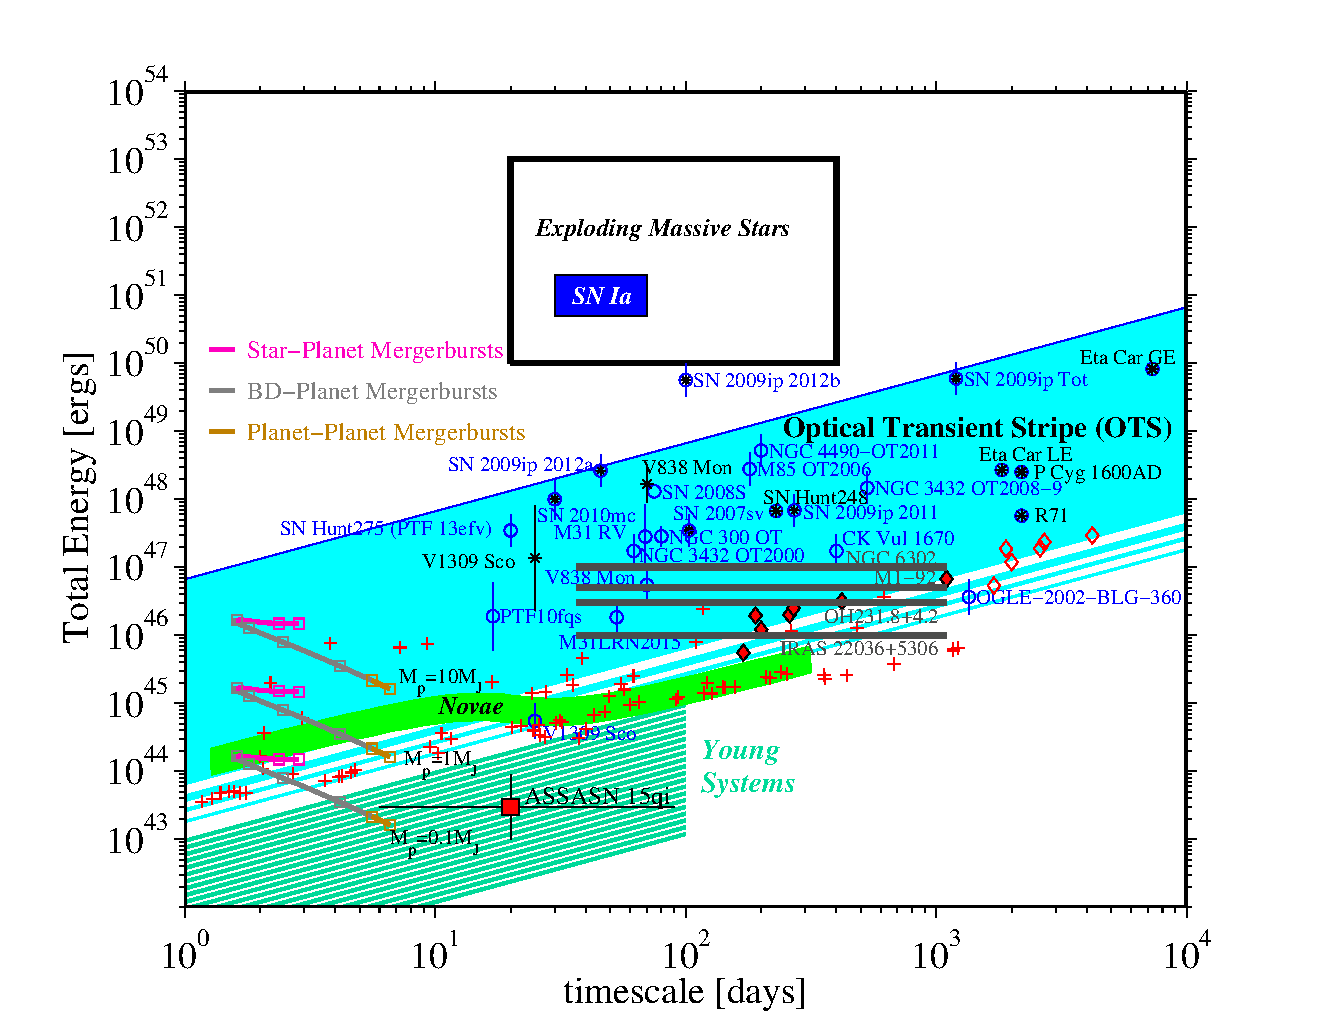
\includegraphics[width=1.0\textwidth]{etd.eps}
    \end{center}
    \caption{
        Energy-Time Diagram (ETD) of observed transient. 
        The Optical Transient Stripe (OTS), is a more or less constant luminosity region in the ETD. 
        It is populated by Intermediate Luminosity Optical Transients (ILOTs). 
        The observed transients include a wide range of objects, probably powered by gravitational energy.
        Some of the objects are merger events or vigorous mass transfer events (see \S\ref{subsec:Types of ILOTs}). 
        Blue empty circles represent the total (radiated plus kinetic) energy of the observed transients as a function of the duration of their eruptions. 
        The duration of an eruption is usually (but not always) defined as the time for the luminosity to decrease by 3 magnitudes $\Delta V=-3$.
        Merger-burst events are marked by blue filled circles.
        The total energy does not include the energy which is deposited in lifting the envelope that does not escape from the star. 
        Where a model exists to calculate the gravitational energy released by the accreted mass (the available energy) it is marked by a black asterisk.
        The supernovae region is schematically marked by a rectangle. 
        The green line represents nova models computed using luminosity and duration from \cite{1995ApJ...452..704D}. 
        Nova models from \cite{2005ApJ...623..398Y} are marked with red crosses, and models from \cite{2010ApJ...725..831S} are represented with diamonds.
        The four horizontal lines are not observed ILOTs, but rather represent the ILOT energy and duration as \cite{2012ApJ...746..100S} modeled for the formation of four bipolar planetary nebulae (PNe) and pre-PNe.
    }\label{fig:etd}
\end{figure}
%%%%%%%%%%%%%%%%%%%%%%%%%%%%%%%%%%%%%%%%%%%%%%%%%%%%%%%%%%%%%%%%%%%%%%%%%%%%%

    \section{Light Curve}

    \section{Summary and Discussion}
    We see also \dots 
    
%%%%%%%%%%%%%%%%%%%%%%%%%%%%%%%%%%%%%%%%%%%%%%%%%%%%%%%%%%%%%%%%%%%%%%%%%%%%%

% \software{astropy \citep{2013A&A...558A..33A},  
%           Cloudy \citep{2013RMxAA..49..137F}, 
%           SExtractor \citep{1996A&AS..117..393B}
%           }

%\appendix

\bibliography{main}{}
\bibliographystyle{aasjournal}

%% Include this line if you are using the \added, \replaced, \deleted
%% commands to see a summary list of all changes at the end of the article.
%\listofchanges

\end{document}
